\documentclass{article}
\usepackage{graphicx} % Required for inserting images
\usepackage[english]{babel}
\usepackage{amsthm}
\usepackage{amsmath}
\usepackage{amsfonts}
\usepackage{tikz}
\usetikzlibrary{matrix}
\usepackage[english]{babel}

\title{MMath project}
\author{Saxon Supple }
\date{January 2024}

\newtheorem{definition}{Definition}
\newtheorem{lemma}{Lemma}
\newtheorem{theorem}{Theorem}

\begin{document}

\maketitle

\section{Singular homology}
\begin{definition}
A \textbf{k-simplex} is the convex hull\\
$[v_0,...,v_k]:=\{\sum_{i=0}^k\lambda_iv_i:\lambda_i\in [0,1],\sum_{i=0}^k\lambda_i=1\}$\\
of $k+1$ linearly independent vectors $v_0,...,v_k\in\mathbb{R}^n$.\\
The \textbf{standard k-simplex} is\\$\Delta^k=[e_0,...,e_k]=\{(t_0,...,t_k)\in\mathbb{R}^k:t_i\geq 0, \sum_{i=0}^kt_i=1\}$\\
The vectors $v_0,...,v_k$ define a \textbf{framing} $F_{v_0,...,v_k}:\Delta^k\rightarrow [v_0,...,v_k],(t_i)\mapsto \sum_{i=0}^kt_iv_i$.
\end{definition}


\noindent For example, $\Delta^0$ is a point, $\Delta^1$ a line segment, $\Delta^2$ a triangle and $\Delta^3$ a tetrahedron.

\begin{definition}
The \textbf{faces} of $[v_0,...,v_k]$ are the (k-1)-simplices $[v_0,...,\overset{\wedge}{v_i},...,v_k]$ where $\overset{\wedge}{v_i}$ means omit the entry $v_i$.
\end{definition}

\begin{definition}
Let $X$ be a topological space. A \textbf{singular k-simplex} in X is a continuous map $\sigma:\Delta^k\rightarrow X$. The \textbf{k-th chain group} of $X$ is the abelian group\\
$C_k(X):=\{\sum_{i=1}^kn_i\sigma_i:k\in\mathbb{N}_0,n_i\in\mathbb{Z},\sigma_i \text{ is a k-simplex}\}$
\end{definition}

\begin{definition}
The \textbf{boundary map} $\partial=\partial_k:C_k(X)\rightarrow C_{k-1}$ is given by\\
$\partial\sigma=\sum_{i=0}^k(-1)^i\sigma\circ F_{e_0,...,\overset{\wedge}{e_i},...,e_k}\in C_{k-1}(X)$\\
on single simplices and extended linearly to all of $C_k(X)$.
\end{definition}
\noindent Intuitively, this definition means that the boundary map decomposes $\sigma$ into a sum of maps to its faces--or rather the images of faces of $\Delta^k$--taking into account orientation.


\begin{lemma}
$\partial\circ\partial:C_k(X)\rightarrow C_{k-2}(x)$ is zero.
\end{lemma}
\begin{proof}
Let $\sigma\in C_k(X)$.\\
$\partial\circ\partial (\sigma)=\partial(\sum_{i=0}^k(-1)^i\sigma\circ F_{e_0,...,\overset{\wedge}{e_i},...,e_k})$\\
$=\sum_{i=0}^k(-1)^i\partial\circ\sigma\circ F_{e_0,...,\overset{\wedge}{e_i},...,e_k}$ by linearity\\
$=\sum_{i=0}^k(\sum_{j<i}(-1)^{i+j}\sigma\circ F_{e_0,...,\overset{\wedge}{e_j},...,\overset{\wedge}{e_i},...,e_k} + \sum_{i<j}(-1)^{i+j-1}\sigma\circ F_{e_0,...,\overset{\wedge}{e_i},...,\overset{\wedge}{e_j},...,e_k})$ (since $e_j$ gets shifted forward one spot when $e_i$ is removed first)\\
$=\sum_{i=0}^k(\sum_{j<i}(-1)^{i+j}\sigma\circ F_{e_0,...,\overset{\wedge}{e_j},...,\overset{\wedge}{e_i},...,e_k} + \sum_{j<i}(-1)^{i+j-1}\sigma\circ F_{e_0,...,\overset{\wedge}{e_j},...,\overset{\wedge}{e_i},...,e_k})$
(interchanging $j$ with $i$ in the second term)\\
$=\sum_{i=0}^k(\sum_{j<i}((-1)^{i+j}+(-1)^{1+j-1})\sigma\circ F_{e_0,...,\overset{\wedge}{e_j},...,\overset{\wedge}{e_i},...,e_k})=0$
\end{proof}

\noindent A simple example of this fact is that the boundary of a ball is a sphere, which in turn has no boundary. It also implies that \\$\text{im}(\partial:C_{k+1}(x)\rightarrow C_k(X))\in\text{ker}(\partial:C_{k}(x)\rightarrow C_{k-1}(X))$,
allowing the following to be well-defined
\begin{definition}
The \textbf{singular homology} of $X$ is the collection of abelian groups
$H_k(X)=\frac{\text{ker}(\partial:C_{k}(x)\rightarrow C_{k-1}(X))}{\text{im}(\partial:C_{k+1}(x)\rightarrow C_k(X))}$
\end{definition}

\section{Proof of the Borsuk-Ulam theorem with cohomology}

\textrm{(Hatcher section 3.2 exercise 3) \\}
We begin with the following lemmas.

\begin{lemma}
There is no map $\mathbb{R} P^n$$\rightarrow$$\mathbb{R} P^m$ inducing a nontrivial map $H^1(\mathbb{R} P^m;\mathbb{Z}_2)\rightarrow H^1(\mathbb{R} P^n;\mathbb{Z}_2)$ if $n>m$.
\end{lemma}
\begin{proof}
Let $x_n$ and $x_m$ be the generators of $H^1(\mathbb{R} P^n;\mathbb{Z}_2)$ and $H^1(\mathbb{R} P^m;\mathbb{Z}_2)$ respectively.

\[H^1(\mathbb{R} P^n;\mathbb{Z}_2)\cong \mathbb{Z}_2\] 
\[H^*(\mathbb{R} P^n;\mathbb{Z}_2)\cong \mathbb{Z}_2[x]/<x^{n+1}>\] 

\noindent Let $f:\mathbb{R} P^n\rightarrow\mathbb{R} P^m $ be such a map so that $f^*(x_m)=x_n$.
Then since $f^*$ is a homomorphism on the cup product structure, $f^*(0)=f^*(x_m^{m+1})=f^*(x_m)^{m+1}=x_n^{m+1}=0$, requiring $m \geq n$. The result follows by contraposition.
\end{proof}

\begin{lemma}
Given any continuous map $f:\mathbb{R}P^n\rightarrow \mathbb{R}P^m$ with $n>m\geq 0$, $f_*:\pi_1(\mathbb{R}P^n)\rightarrow \pi_1(\mathbb{R}P^m)$ is trivial.
\end{lemma}
\begin{proof}
 $f^*:H^1(\mathbb{R}P^m;\mathbb{Z}_2)\rightarrow H^1(\mathbb{R}P^n;\mathbb{Z}_2)$ is dual to $f_*:H_1(\mathbb{R}P^n;\mathbb{Z}_2)\rightarrow H_1(\mathbb{R}P^m;\mathbb{Z}_2)$ which is equal to $f_*:\pi_1(\mathbb{R}P^n)\rightarrow \pi_1(\mathbb{R}P^m)$ by the Hurewicz theorem and the fact that $\pi_1(\mathbb{R}P^k)$ is abelian. Thus $f_*$ is trivial by the above result.
\end{proof}

We are now able to prove the main theorem.
\begin{theorem}
\textbf{Borsuk-Ulam theorem:} For integers $n>m\geq 0$ there is no continuous map $\phi:S^n\rightarrow S^m$ which is antipode preserving, meaning $\phi(-x)=-\phi(x)$ for all $x$.
\end{theorem}
\begin{proof}
Suppose that there exists a continuous antipode preserving map $\phi:S^n\rightarrow S^m$. Define $\psi:\mathbb{R}P^n\rightarrow \mathbb{R}P^m$ by $\psi([x])=[\phi(x)]$. $\psi$ is well-defined since $x\sim y \implies x=\pm y \implies \phi(x)=\pm\phi(y) \implies \phi(x)\sim\phi(y)$. $\psi$ is also continuous by the universal property of quotients for the quotient map $p:S^k\rightarrow \mathbb{R}P^k$.
Fix $x\in S^n$ and let $y=\phi(x)$. $\psi_*:\pi_1(\mathbb{R}P^n,[x])\rightarrow \pi_1(\mathbb{R}P^m,[y])$ is trivial by the above lemma, so has a unique lift $\psi':(\mathbb{R}P^n,[x])\rightarrow (S^m,y)$ under the covering map $p$ by the ultimate lifting theorem. This gives a commutative diagram

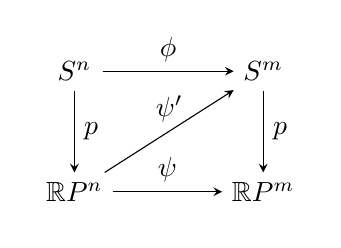
\begin{tikzpicture}
  \matrix (m) [matrix of math nodes,row sep=3em,column sep=4em,minimum width=2em] {
     S^n & S^m \\
     \mathbb{R}P^n & \mathbb{R}P^m \\};
  \path[-stealth]
    (m-1-1) edge node [right] {$p$} (m-2-1)
            edge  node [above] {$\phi$} (m-1-2)
    (m-2-1.east|-m-2-2) edge  node [above] {$\psi$} (m-2-2)
    (m-1-2) edge node [right] {$p$} (m-2-2)
            (m-2-1) edge  node [above]{$\psi'$} (m-1-2);
\end{tikzpicture}
\\
$\psi' \circ p$ and $\phi$ are both lifts of $\psi \circ p$ and both map $x\mapsto y$ so $\phi = \psi'\circ p$ by uniqueness. But then $\psi'(p(-x))=\psi'([x])=y=\phi(x)$, contradicting $\phi(-x)=-y$.
\end{proof}

\end{document}
